\section{Simulations}

Our experiments apply feedback alignment algorithm to a two-layer network training on both synthetic and real-world data, where a range of the networks with different network width and activations are considered. The results illustrate that the regularizations are essential to both regression and classification task.

\paragraph{Feedback alignment on synthetic dataset.}

We first train a two-layer network on synthetic data. The network $f$ has the form as in \eqref{eqn:nonlinear-network} and the data is generated by another network $f_0$ that has the same form as $f$ but randomly generated weights. We present the experiments for both linear and nonlinear network, where the activations are chosen to be ReLU and Tanh for nonlinear case. We set training sample $n=50$ and input dimension $d=150$ but vary the hidden layer width $p = 100\times 2^i$ with $i\in[7]$. 


\begin{figure}[h]
\centering
\begin{subfigure}[b]{.33\textwidth}
  \centering
  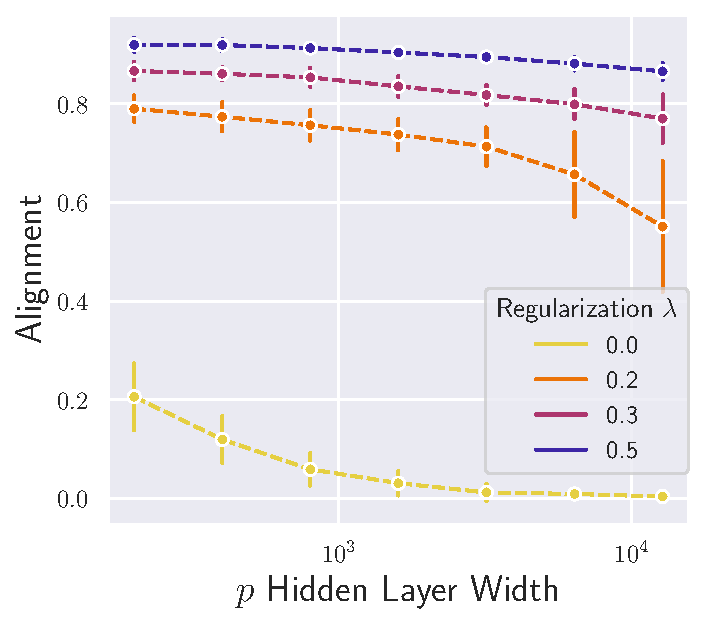
\includegraphics[width=\linewidth]{figures/df_lr_non_autograd_l2_v6.pdf}
  \caption{Alignment on linear network.}
  \label{fig:align_lr_non_autograd_l2}
\end{subfigure}\hfill
\begin{subfigure}[b]{.33\textwidth}
  \centering
  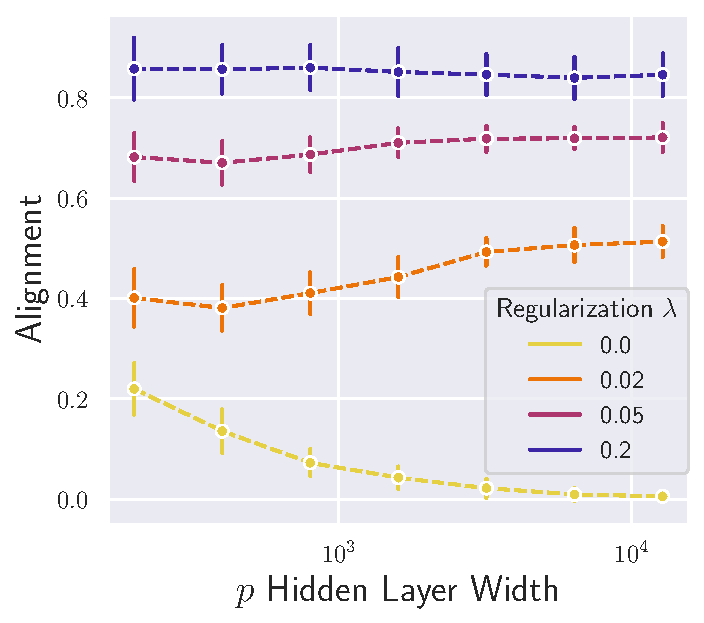
\includegraphics[width=\linewidth]{figures/df_nn_relu_autograd_l2_v6.pdf}
  \caption{Alignment on ReLU network.}
  \label{fig:align_nn_relu_autograd_l2}
\end{subfigure}\hfill
\begin{subfigure}[b]{.33\textwidth}
  \centering
  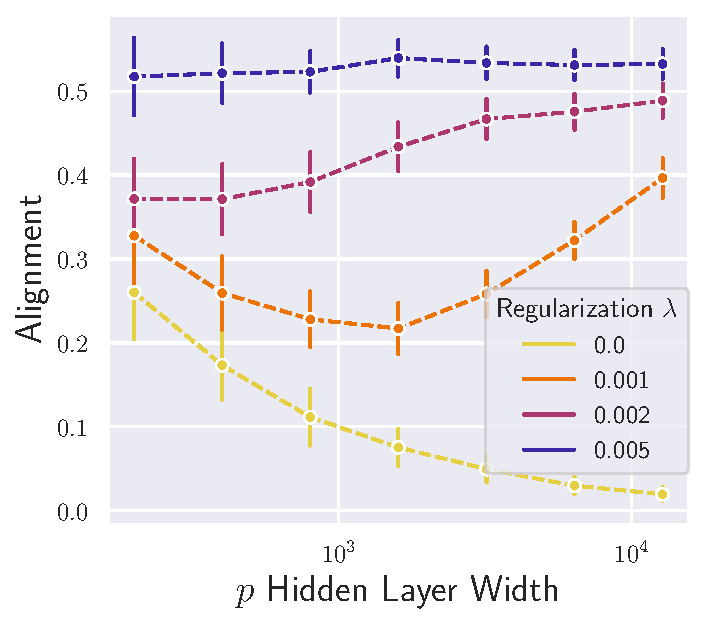
\includegraphics[width=\linewidth]{figures/df_nn_tanh_autograd_l2_v6.pdf}
  \caption{Alignment on Tanh network.}
  \label{fig:align_nn_tanh_autograd_l2}
\end{subfigure}
\medskip
\begin{subfigure}[b]{.33\textwidth}
  \centering
  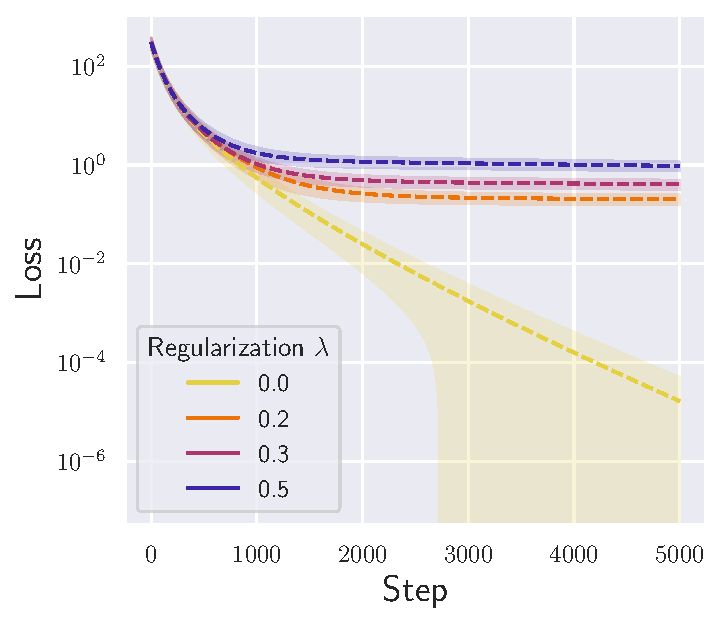
\includegraphics[width=\linewidth]{figures/loss_lr_non_autograd_l2_v1.pdf}
  \caption{Loss on linear network.}
  \label{fig:loss_lr_non_autograd_l2}
\end{subfigure}\hfill
\begin{subfigure}[b]{.33\textwidth}
  \centering
  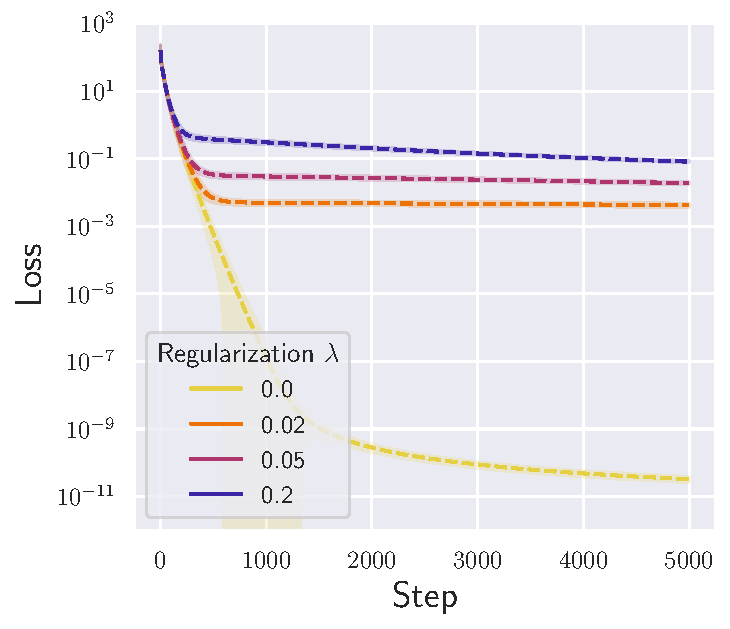
\includegraphics[width=\linewidth]{figures/loss_nn_relu_autograd_l2_v1.pdf}
  \caption{Loss on ReLU network.}
  \label{fig:loss_nn_relu_autograd_l2}
\end{subfigure}\hfill
\begin{subfigure}[b]{.33\textwidth}
  \centering
  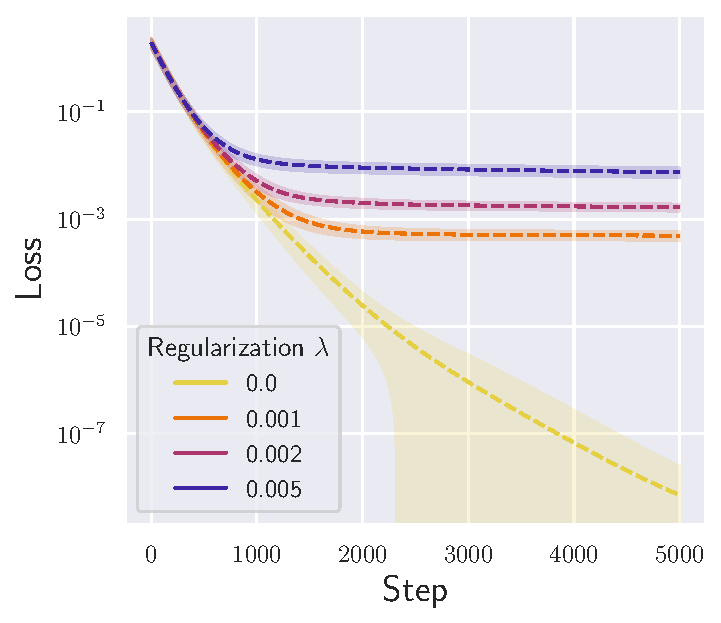
\includegraphics[width=\linewidth]{figures/loss_nn_tanh_autograd_l2_v1.pdf}
  \caption{Loss on Tanh network.}
  \label{fig:loss_nn_tanh_autograd_l2}
\end{subfigure}
\caption{Comparisons on the alignment for feedback alignment algorithm with different levels of $\ell_2$ regularization. In each figure, the $x$-axis denotes the width $p$ of hidden layer, and it is in logarithmic scale; the $y$-axis represents the level of alignment as the normalized inner product between $\beta_t$ and $b$. The data points are the mean value computed across simulations, and the error bars mark the standard deviation among different runs.}
\label{fig:synthetic-l2}
\end{figure}

In \cref{fig:synthetic-l2} we show numerically how alignment depends on regularization and the hidden layer width $p$, where the alignment is measured by the cosine of the angle between forward weights $\beta$ and backward weights $b$. During training, we take step size $\eta = 10^{-4}$ for linear networks and $\eta = 10^{-3},10^{-2}$ for ReLU and Tanh networks, respectively. We train the network until converge and this procedure is repeated $50$ times for each $p$ and $\lambda$. It can be observed that for all three types of networks, as $p$ goes large, alignment is vanishing if there is no regularization, while alignment is stably away from zero if regularization is added. Further, alignment grows along with the level of regularization $\lambda$ for the same network. Such numerical results are highly consistent to our theoretical statements.

We would like to remark that dropout, a commonly used training technique, as a form of regularization can also help the alignment between forward and backward weights when used together with feedback alignment algorithm \citep{wager2013dropout}. To the best of our knowledge, there is no satisfying theoretical result available that could explain the underlying mechanism.


\paragraph{Feedback alignment on MNIST dataset.}

The training set of \texttt{MNIST} data consists of $6000$ black-and-white images of handwritten digits with dimension $28$ by $28$, and we reshape each of them into an one-dimensional vector of length $d = 784$. The training data $x_i$'s are obtained after normalizing the vectors by their mean and standard deviation. The test dataset with $1000$ samples can be similarly processed. We remark that the structure of the two-layer ReLU network we use for classification has a different output size compared to \eqref{eqn:nonlinear-network}. In particular, the output dimension for \texttt{MNIST} classification is $10$ instead of $1$, and we utilize cross-entropy loss on evaluating the predictions against the categorical labels $y$. During training, we choose a batch size $n = 600$ and there are $100$ steps taken within each epoch with step size $\eta = 10^{-2}$. The training procedure takes $300$ epochs in total. 

\cref{fig:mnist} shows the performance of (regularized) feedback alignment under regularization $\lambda = 0, 0.1, 0.3$. The figure on the right-hand side shows the change on test accuracy for different classifiers during training, and the networks trained with regularization are able to outperform the one without regularization. The regularized feedback alignment quickly converges to the maximum accuracy for larger regularization $\lambda$. In the first two figures, we show the development of alignment during feedback alignment training procedure, and it grows faster with larger regularization. Recall that the second layer weights $\beta\in\RR^{p\times 10}$ is not a vector, and under such scenario the definition of alignment between backpropagated error signals $\dfa$ and $\dbp$ is no longer equivalent to that in \cref{def:alignment}. The first plot follows the definition from \citep{lillicrap2016random} and the second one follows \cref{def:alignment}, and it turns out they are very close to each other numerically.

\begin{figure}[t]
  \centering
  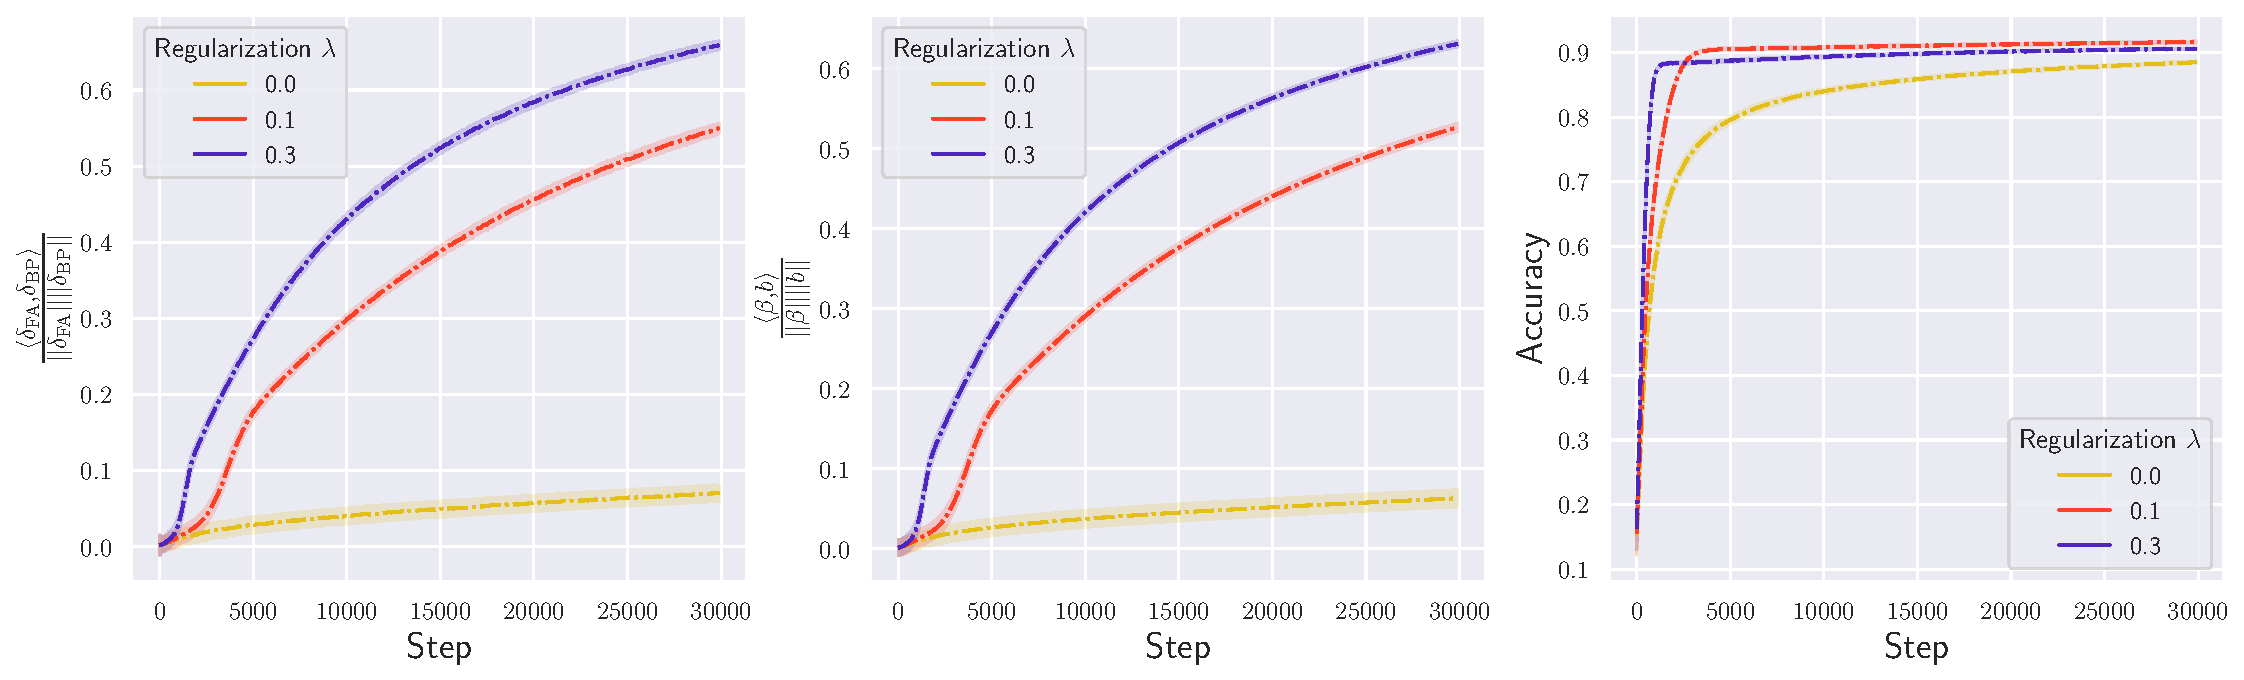
\includegraphics[width=\textwidth]{figures/mnist_2l_v6_horizontal.pdf}
  \caption{Comparisons on alignment and accuracy for feedback alignment algorithm with different levels of $\ell_2$ regularization. In each of the three plots, the $x$-axis represents the number of updates on model parameters. In particular, the $y$-axes in the left and the middle plots show two notions of alignment: alignment of backpropagated error signals and alignment of forward and backward weights, respectively. The plot on the right shows the accuracy achieved by networks on test dataset. The dashed lines and corresponding shaded areas represent the means and the standard deviations over $10$ runs with random initialization.}
  \label{fig:mnist}
\end{figure}